\section{Model logiczny w postaci bramek}
\label{sec:bramki}

\subsection{Równanie stanu}
Zachowanie przerzutnika T z zerowaniem można opisać zależnością:
\begin{equation}
    Q_{\text{next}} \;=\; \bigl(P \oplus Q\bigr) \,\land\, \lnot T ,
    \label{eq:main}
\end{equation}
gdzie $P = S_1 \lor S_2 \lor S_3 \lor S_4$, a $T$ jest sygnałem
przekroczenia dopuszczalnego czasu bezruchu.

\subsection{Schemat bramkowy}
Rysunek~\ref{fig:bramki} przedstawia realizację równania~\eqref{eq:main}
przy użyciu bramek OR, XOR, AND oraz NOT.

\begin{figure}[H]
\centering
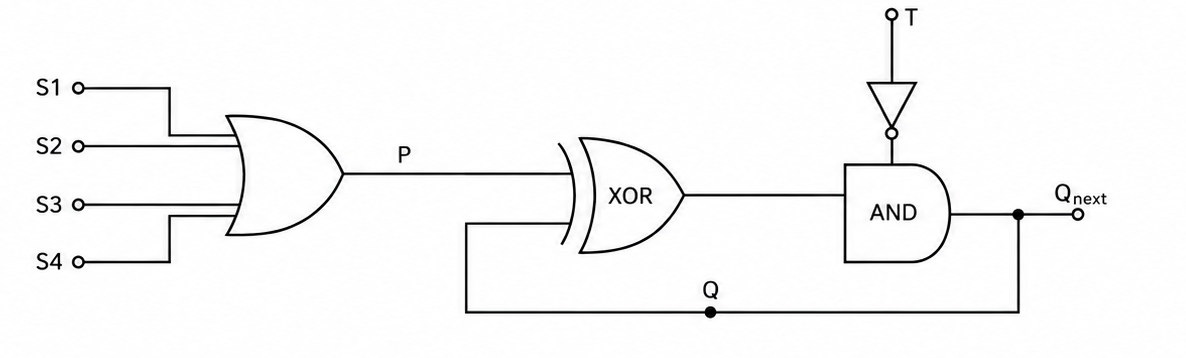
\includegraphics[width=\textwidth]{figures/Blokowy.png}
\caption{Schemat logiczny układu sterowania oświetleniem.}
\label{fig:bramki}
\end{figure}